\documentclass[12pt, twoside]{article}
\usepackage[francais]{babel}
\usepackage[T1]{fontenc}
\usepackage[latin1]{inputenc}
\usepackage[left=4mm, right=4mm, top=4mm, bottom=4mm]{geometry}
\usepackage{float}
\usepackage{graphicx}
\usepackage{array}
\usepackage{multirow}
\usepackage{amsmath,amssymb,mathrsfs} 
\usepackage{soul}
\usepackage{textcomp}
\usepackage{eurosym}
\usepackage{lscape}
 \usepackage{variations}
\usepackage{tabvar}
 
\pagestyle{empty}

\title{\ul{\textbf{Activit�: p�rim�tre et aire d'une figure}}}
\date{}

\begin{document}
\maketitle


\section{Quelques rappels}

\subsection{P�rim�tre}

\ul{D�finition}: Le p�rim�tre d'une figure est la longueur du contour de cette
figure.



\begin{center}
\begin{tabular}{|c|c|c|c|c|c|c|}
\hline
 \qquad \qquad & \qquad \qquad & \qquad \qquad & \qquad \qquad & \qquad \qquad &
 \qquad \qquad & \qquad \qquad \\
 \hline
\end{tabular}
\end{center}



\ul{Exemple:} 

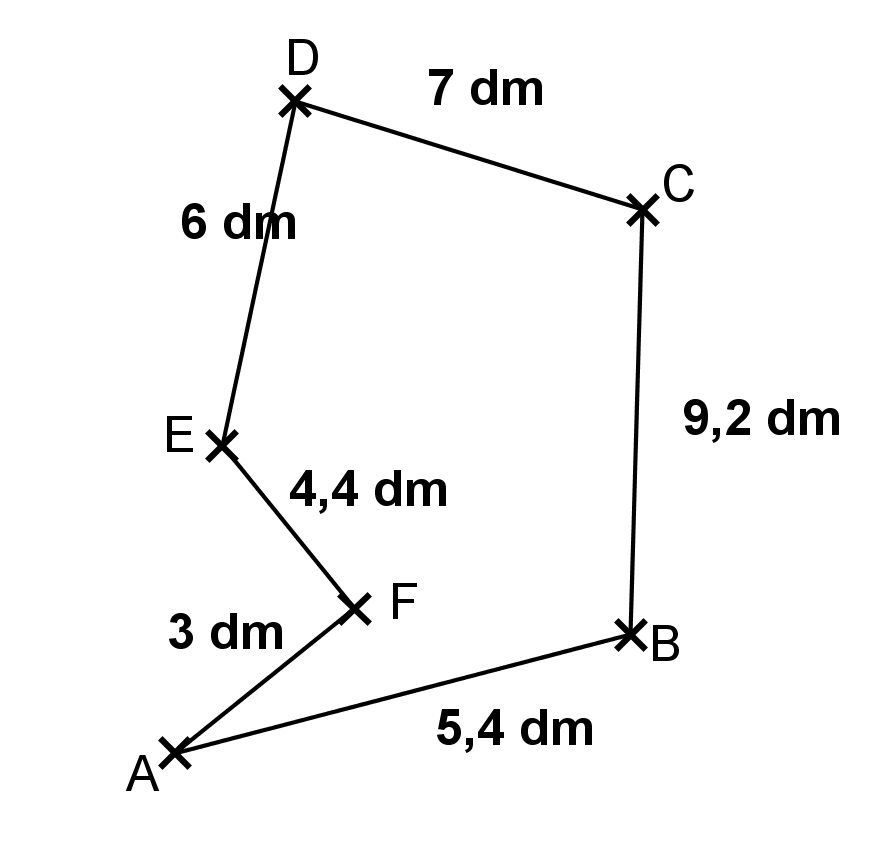
\includegraphics[width=40mm]{images/perimetre.png} 
 


\subsection{Aire}


\begin{center} 
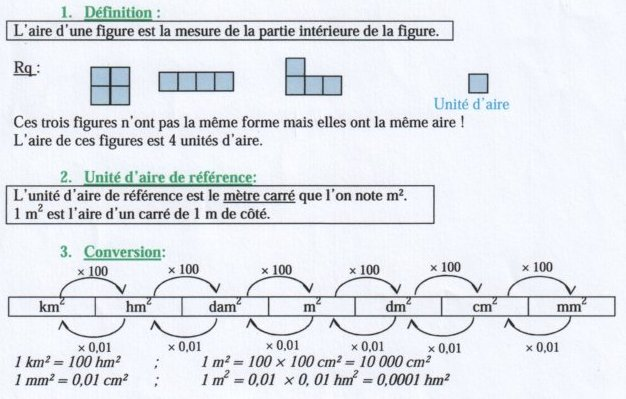
\includegraphics[width=12cm]{images/aire.jpg}
\end{center}


\ul{Exemples}:
\quad $325 m^2=\ldots \ldots \ldots cm^2$  \qquad \qquad \qquad \qquad $17
hm^2=\ldots \ldots km^2$



\subsection{Le nombre $\pi$}



La lettre grecque $\pi$ se lit ``pi''. $\pi$ est la lettre grecque qui
correspond au \textbf{p} de notre alphabet.

\enskip


Le nombre $\pi$ n'est pas d�cimal; il a un nombre  \textbf{infini} de chiffres
apr�s la virgule. La touche \fbox{$\pi$} de la calculatrice en donne une valeur
approch�e: 3,141592654\ldots


\section{Formulaire}

\ul{\textbf{P�rim�tre}}

\enskip

Carr� \qquad \qquad \qquad \qquad \qquad \qquad Rectangle \qquad \qquad \qquad
\qquad \qquad \qquad Cercle

\bigskip

\bigskip

\bigskip

\bigskip

\bigskip


\ul{\textbf{Aire}}

\enskip


Carr� \qquad \qquad \qquad Rectangle \qquad \qquad \qquad Triangle rectangle
\qquad \qquad \qquad Triangle \qquad \qquad \qquad Disque

\bigskip

\bigskip

\bigskip

\bigskip

\bigskip

\bigskip





\bigskip




\section{A vous de jouer\ldots}

\begin{tabular}{cc}
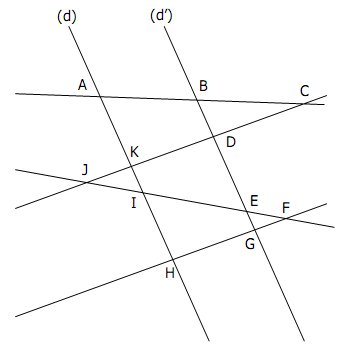
\includegraphics[width=8cm]{images/ex1.jpg} 
&
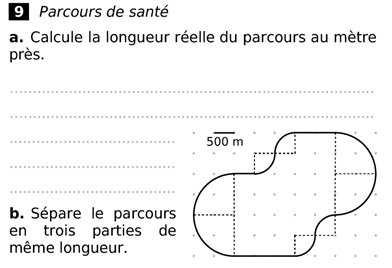
\includegraphics[width=9cm]{images/ex2.jpg} \\
\end{tabular}


\bigskip


\begin{tabular}{cc}
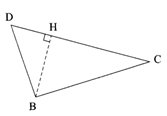
\includegraphics[width=8cm]{images/ex4.jpg}
&
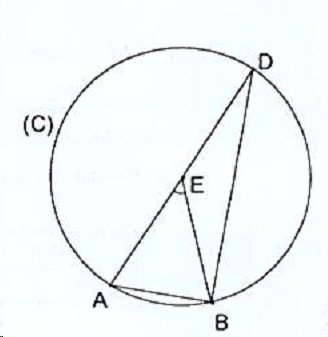
\includegraphics[width=9cm]{images/ex3.jpg}\\

\end{tabular}



\end{document}
